\section{Background}
\label{sec:background}

%===================Background=====================%

% While it is conventional for the operating system kernel to handle page faults, delegating page fault handling to the userspace has proven to be more flexible in some use cases (in some impactful projects.)

While page faults are traditionally handled by the kernel, in some cases it is beneficial to let applications customize page fault handling. For example, virtual machine (VM) live migration allows virtual clusters to migrate VMs across physical hosts with minimal disruption to the guest~\cite{vm-migration}. It is an important capability, commonly used for VM/host software upgrades, load balancing, hardware failure handling, and scheduled maintenance~\cite{google-live-migration-at-scale}.
When using the post-copy migration strategy, most of the VM's memory gets copied on-demand, thereby minimally impacting the application~\cite{post-copy, bare-metal-post-copy}. A similar technique can be used for checkpoint-restore-in-userspace (CRIU), which saves a process's state to disk and restores it at a later point \cite{CRIU_Userfaultfd}. When a process is restored, rather than copying its entire state to its address space, relevant pages can be copied on-demand, reducing start-up time. While such functionality could be supported through significant kernel modifications~\cite{post-copy}, a more general-purpose solution is desirable.

%\asaf{List several examples of applications that use userfaultfd today and in a few words say how they use it} \teng{Maybe observablity projects, zIO, ...}To provide background on user page fault handling, for the rest of the section we use a guiding example of post-copy virtual machine (VM) migration~\cite{post-copy}.

% Pre-copy copies states including memory. Post-copy copies states except memory.
%There are two main live migration techniques: pre-copy and post-copy migration. Pre-copy copies all the VM state to the destination, while post-copy only copies the VM's memory pages on-demand, which brings better performance in terms of migration downtime. According to Im et al.\ \cite{bare-metal-post-copy}, post-copy migration reduces downtime by orders compared to pre-copy migration when running a Redis Workload. 
%MFN swapping and need support from the hypervisor to xxx page fault handling.

%Initially, there were several methods to detect and trap page faults for post-copy migration at the target VM, including shadow paging and pseudo paging, both of which require significant kernel code modification \cite{post-copy}. With the introduction of $\texttt{userfaultfd()}$ syscall in the Linux kernel \teng{when, cite source}, applications can finally retrieve remote pages with a customized, user-space, easy-to-implement page fault handler.

%===================uffd mechanism breakdown=====================%

To solve this problem, Linux introduced the \texttt{userfaultfd()} syscall, allowing applications to handle page faults in userspace with an additional fault-handling thread~\cite{kernel_userfaultfd, uffd_presentation}. We illustrate a \texttt{userfaultfd()} workflow with CRIU as an example use case in Figure~\ref{fig:live-migration-diagram}.

\begin{figure}
    \centering
    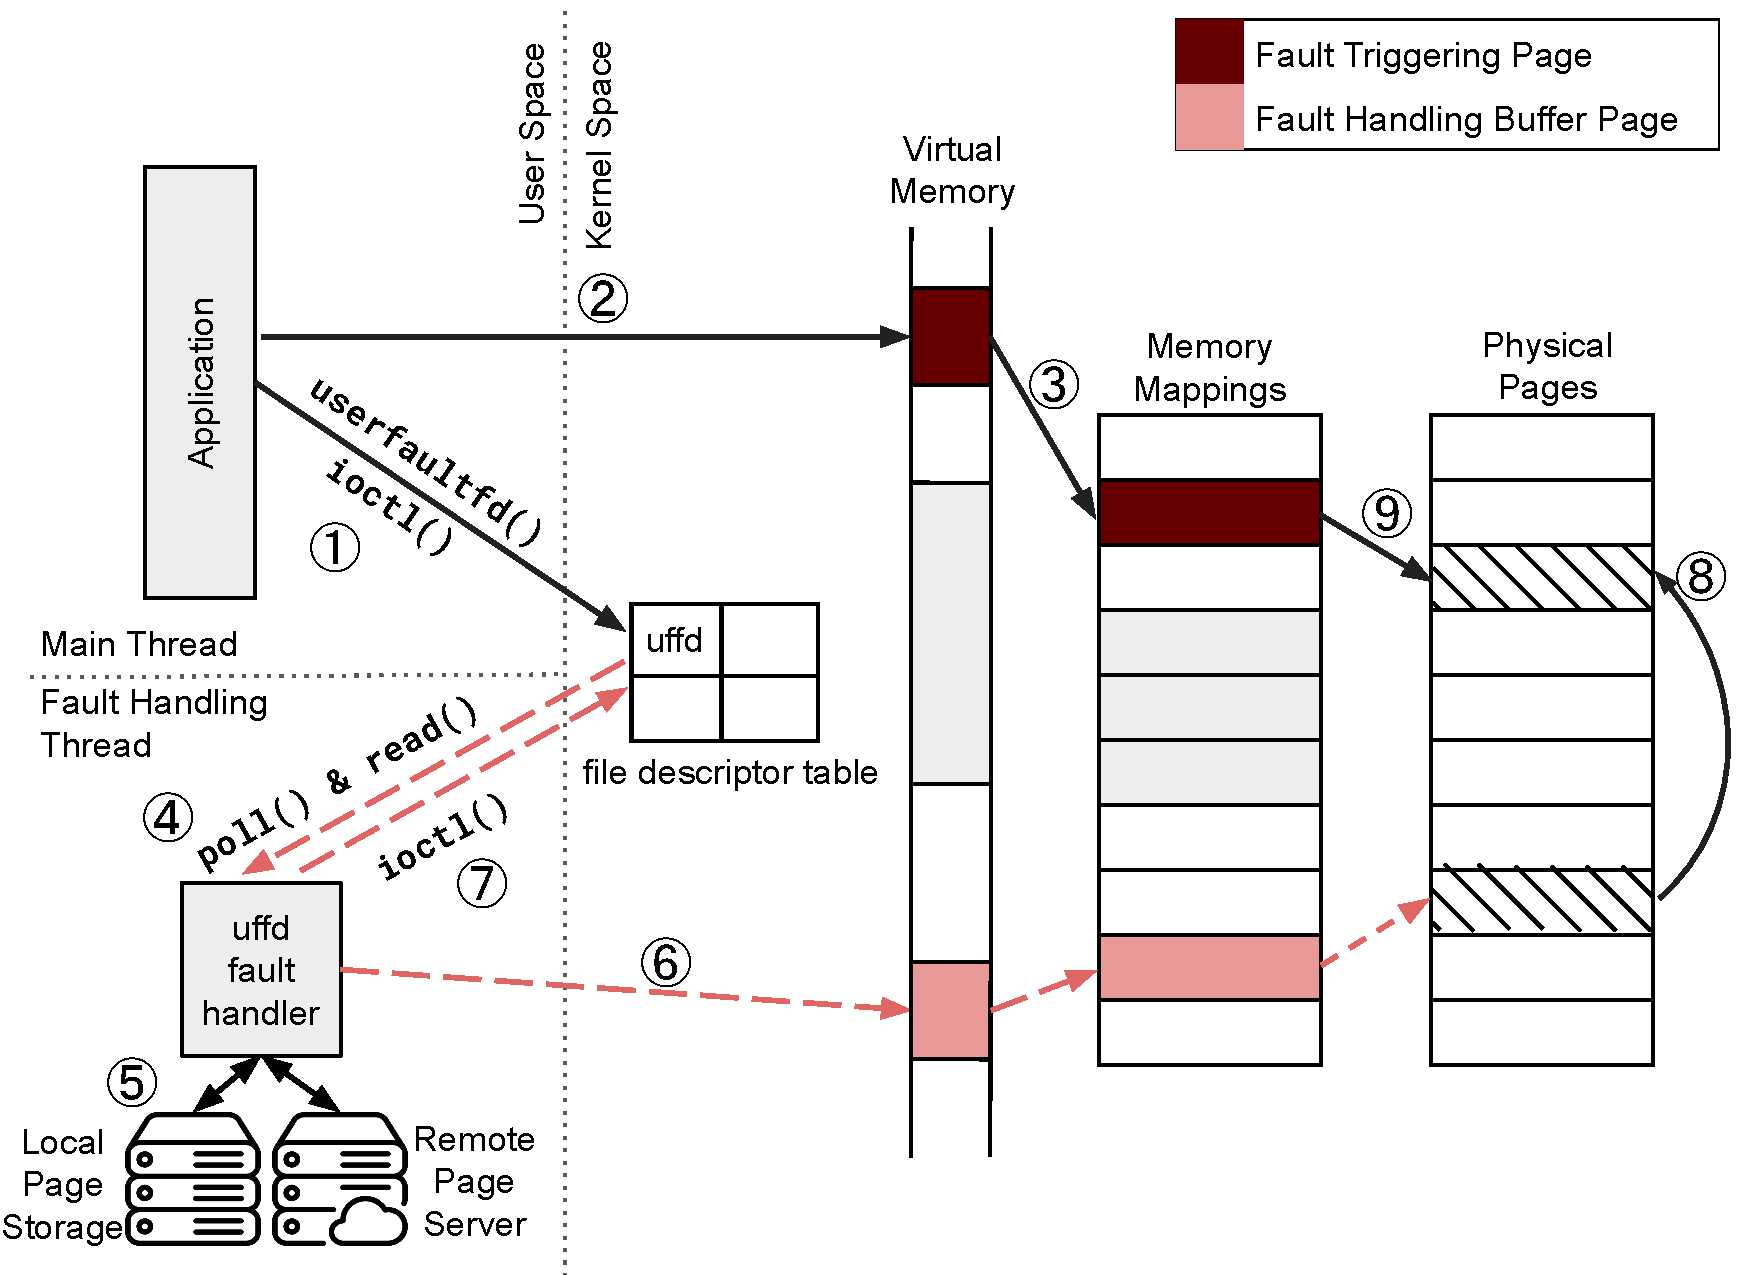
\includegraphics[clip,scale=0.26]{figures/uffd-v7.0.pdf}
    \caption{\texttt{userfaultfd()} workflow. }
    \label{fig:live-migration-diagram}
    %\vspace{-2em}
\end{figure}

% This corresponds to the "Local Page Storage" and "Remote Page Server"
Assuming we want to restore an application to a checkpointed state (\ie its state is stored on a local or remote disk), the CRIU client sets up an initial subset of the application's pages. The remaining pages aren't initialized yet, as we want to copy them the first time the application tries to access them, requiring a custom page fault handler. The CRIU client then calls \texttt{userfaultfd()}, creating a new uffd (userfault file descriptor), and uses \texttt{ioctl()} to register the regions of virtual memory (the application's remaining pages) it should handle (\pgftextcircled{1}). After creating a fault-handling thread that polls on the uffd, the application can safely resume execution.
When the application attempts to access an unmapped page (\pgftextcircled{2} and \pgftextcircled{3}), a page fault is raised. If the relevant page is in a \texttt{userfaultfd()}-registered region, the kernel marks the uffd as ready, waking up the fault-handling thread, which then reads from the uffd (\pgftextcircled{4}). For CRIU, the fault-handling thread will read the relevant data from the application's (local or remote) checkpoint (\pgftextcircled{5}) into a local buffer (\pgftextcircled{6}). The thread then submits a \texttt{userfaultfd()} command using \texttt{ioctl()} (\pgftextcircled{7}), which atomically copies the data into the application's address space, resolving the fault (\pgftextcircled{8}, \pgftextcircled{9}).

%Suppose we have an application we want to checkpoint. On the source side, we can either dump the memory to local disk or start a page server for the restored application to listen to requests of pages over the network, illustrated on the bottom left of Figure \ref{fig:live-migration-diagram}.
%On the restorer side,  we use \texttt{userfaultfd()} to create a new uffd (userfault file descriptor) and use the \texttt{ioctl()} system call with different flags to learn about available features and register one or more regions of virtual memory with certain kinds of page fault. At the same time, we create a fault-handling thread that polls on the uffds.

%Once a fault occurs in certain memory regions (\pgftextcircled{1} and \pgftextcircled{2} in Figure \ref{fig:live-migration-diagram}), the fault-handling thread will be woken up. It will either connect to the remote page server or read from local files to fill up a buffer page, then call \texttt{ioctl()} again with certain flags (usually \texttt{UFFDIO\_COPY}, which notify the fault triggering thread to copy (\pgftextcircled{4}) the buffer page to the faulting page (\pgftextcircled{5}, \pgftextcircled{6}, \pgftextcircled{7})). Finally, the application can access the content of the page ((\pgftextcircled{3}).

% \asaf{maybe guide this description (and also the rest of the paper) with an example of a specific application}

% Firecracker \cite{firecracker} provides a better management of the microVM's memory loading by letting users choose between relying on the host OS to handle the page faults when resuming from a snapshot, or having a dedicated userspace process for dealing with page faults, with the help of Userfaultfd.

%While \texttt{userfaultfd()} supports other modes, such as tracking minor faults and write-protected pages, we primarily focus on its major fault functionality.

In addition to CRIU, \texttt{userfaultfd()} has seen adoption in a number of large projects, along with more experimental work \cite{zIO, LightSwap, file-backed-article, file-backed-proceeding, uffd-security-framework-paper, TrailDB}. \texttt{userfaultfd()} is used by QEMU for VM post-copy migration, while Firecracker uses it to lazily restore microVM memory from a snapshot~\cite{firecracker}. The Android Runtime's garbage collector uses \texttt{userfaultfd()} in its compaction phase to track page accesses~\cite{Android_13_AOSP, garbage_collection_paper}.
Additionally, the authors of \texttt{userfaultfd()} have identified several additional potential use cases, such as distributed shared memory, language runtimes, and JIT compilers, along with adding support for handling write-protect and minor faults~\cite{LWN_Write-protect, LWN_next_step, LPC-presentation, uffd_presentation}.
Finally, we believe that there exist additional use cases for custom page fault handling which cannot utilize \texttt{userfaultfd()} due to its limitations, such as lazily resolving data relocations for position-independent executables in the dynamic linker, yielding faster program start-up~\cite{chromium-elf}.
We discuss these limitations in Section~\ref{sec:motivation}.

%A lot of other applications also benefit from the flexibility of customized page fault handling. Utilizing \texttt{userfaultfd()}, UMap\cite{file-backed-article, file-backed-proceeding} designs an interface akin to mmap but with faster access to large files. Lightswap \cite{LightSwap} enhances the performance of the swapping system. A lot of other work \cite{zIO, } also performs page fault interception. Some other user cases for memory observability.
